\chapter{Related Work}\label{chapter:related}

\section{Nikolas Schneider}

\begin{figure}[h]
\centering
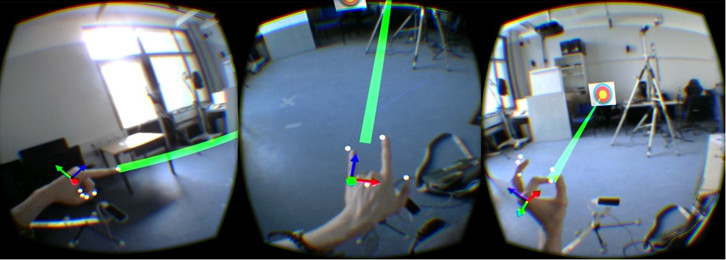
\includegraphics[width=\textwidth]{nick}
\caption{Nikolas Schneider: Pointing, Spiderman and Pinching Posture}
\label{fig:Nick}
\end{figure}

Being its follow-up work, this bachelor thesis was highly influenced by the work of Nikolas Schneider \cite{schneider_2016}. In his bachelor thesis Nikolas Schneider compared three different hand postures, namely a pointing, spiderman and a pinching posture in terms of precision and performance in a 3D-pointing task (Figure \ref{fig:Nick}). 

For that, he conducted a user study, where the participants had to perform a target shooting test in a Unity 3D environment using one of the mentioned postures. For that purpose the participants wore an AR-Rift giving them augmentations of the targets to shoot and the shooting direction, indicated by a laser beam. The beam's origin and direction were computed differently for each hand posture.  In order to track the participant's hand, a metal construction featuring a Leap Motion Controller and ART marker was strapped to the forearm. Applying a KNN algorithm on the data gained from the Leap, the user's hand posture was determined in order to make sure, the participant would hold the posture throughout the test. Right after the target shooting, users were asked to rate their experience with the hand postures regarding perceived accuracy and comfort. 

The results showed that generally the pointing posture performed best, followed by the spiderman posture and finally the pinching posture. The questionnaire revealed similar results for user perception, indicating a connection between user comfort and performance.

\section{Comfort and Discomfort}

As the main goal was to create a quantitative metric for hand posture comfort and discomfort evaluation, it was crucial to understand state of the art concepts of comfort and discomfort and to have a look at similar approaches taken to create comfort metrics.

In their editorial Vink et al. \cite{vink2012editorial} give a good overview over current comfort and discomfort definitions, different models explaining the origin of both. They state that even though there has been much research on comfort and discomfort, the results are generally ignored in practical design contexts due to their broad theoretical scope. Concluding they express the importance of further research in order to generate applicable models and metrics for concrete body parts.

Fagarasanu et al. \cite{fagarasanu2004measurement} discovered that limbs in neutral postures showed a significantly lower muscle activity, indicating higher perceived comfort. Apostolico et al. \cite{apostolico2014postural} defined the term "Range of Rest Posture" (RRP), a angular range for articular joints where the joint can be seen as statistically in rest. They further measure the RRP for multiple human joints and express its importance for evaluation of postural comfort. Based on this, Naddeo et al. \cite{naddeo2015proposal} used a neural network to generate a concrete metric for postural comfort based on RRP. Therefore they compare user comfort ratings of certain joint postures with the measured distance to the RRP. They further also described other potential influential factors to take into account when evaluating comfort.

Short et al. \cite{short1999precision} conducted a user study to investigate the so called precision hypothesis. The results indicated that generally more comfortable posture generate a higher precision in pointing tasks. This effect is magnified, when the targets become smaller.